% diagrams/nino-perro-jardin.tex -- un niño y un perro en el jardín (línea, para colorear).
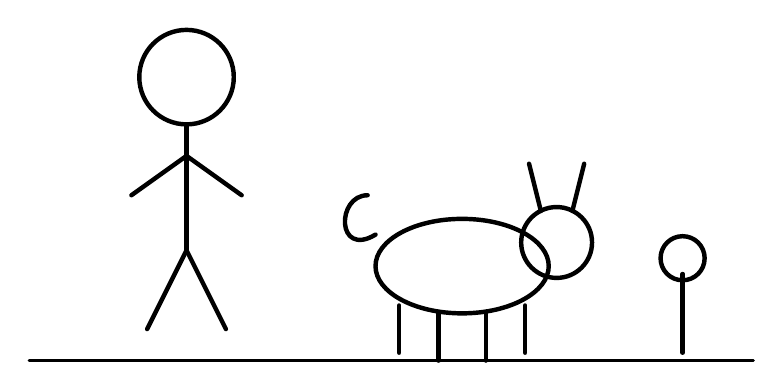
\begin{tikzpicture}[line width=1.6pt, line cap=round, line join=round]
  % niño
  \draw (-3,0.4) circle (0.6);
  \draw (-3,-0.2) -- (-3,-1.8);
  \draw (-3,-0.6) -- (-3.7,-1.1);
  \draw (-3,-0.6) -- (-2.3,-1.1);
  \draw (-3,-1.8) -- (-3.5,-2.8);
  \draw (-3,-1.8) -- (-2.5,-2.8);
  % perro: cuerpo
  \draw (0.5,-2) ellipse (1.1 and 0.6);
  % patas
  \draw (-0.3,-2.5) -- (-0.3,-3.1);
  \draw (0.2,-2.6)  -- (0.2,-3.2);
  \draw (0.8,-2.6)  -- (0.8,-3.2);
  \draw (1.3,-2.5)  -- (1.3,-3.1);
  % cabeza y orejas
  \draw (1.7,-1.7) circle (0.45);
  \draw (1.5,-1.3) -- (1.35,-0.7);
  \draw (1.9,-1.3) -- (2.05,-0.7);
  % cola
  \draw (-0.6,-1.6) .. controls (-1.1,-1.9) and (-1.1,-1.1) .. (-0.7,-1.1);
  % flor sencilla, para el jardín
  \draw (3.3,-3.1) -- (3.3,-2.1);
  \draw (3.3,-1.9) circle (0.28);
  % suelo
  \draw[line width=1pt] (-5,-3.2) -- (4.2,-3.2);
\end{tikzpicture}
